% Une ligne commentaire débute par le caractère « % »

\documentclass[a4paper]{article}

% Options possibles : 10pt, 11pt, 12pt (taille de la fonte)
%                     oneside, twoside (recto simple, recto-verso)
%                     draft, final (stade de développement)

\usepackage[utf8]{inputenc}   % LaTeX, comprends les accents !
\usepackage[T1]{fontenc}      % Police contenant les caractères français
\usepackage[francais]{babel}  


\usepackage[a4paper,left=2cm,right=2cm]{geometry}% Format de la page, réduction des marges
\usepackage{graphicx}  % pour inclure des images

%\pagestyle{headings}        % Pour mettre des entêtes avec les titres
                              % des sections en haut de page

 \title{  Qui est-ce ?\\         % Les paramètres du titre : titre, auteur, date
  Projet de programmation}          
\author{Groupe \emph{Z}\\
  \emph{Frédéric,Laurent,Tony et Romain}\\
  \emph{git:git@gitlab.etu.umontpellier.fr:e20180001091/qui-est-ce.git}\\
  L2 informatique\\
  Faculté des Sciences\\
Université de Montpellier.}
\date{\today}             


\begin{document}

\maketitle                    % Faire un titre utilisant les données
                              % passées à \title, \author et \date

\begin{center}               % pour centrer 
  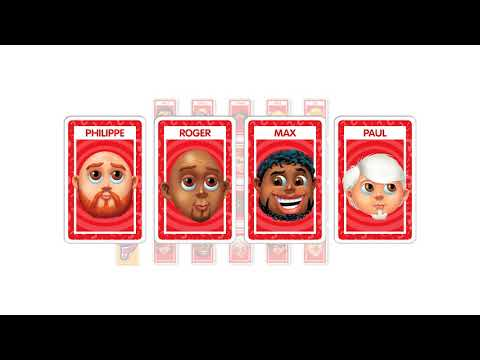
\includegraphics[scale=1]{img.jpg}   % insertion d'une image
\end{center}

\begin{abstract}     % Résumé du travail

  \emph{Description très succinte du problème et des différentes étapes de réalisation}

\end{abstract}


\section{ Technologies utilisées  et organisation} % Commencer une section, etc.

\emph{Une page.}

\subsection{Choix du langage}         % Section plus petite

\begin{itemize}            % Liste non numérotée
\item
  Le langage que vous avez choisi d'utiliser.
\item
  Bibliothèques, framework, ... utilisés
\end{itemize}

\subsection{Organisation du travail}

\begin{enumerate}           % Liste numérotée
\item
  Répartition du travail au sein du groupe
\item
  Rythme de travail, mode de fonctionnement ...
\end{enumerate}
\section{Étape 1 : permettre à l'utilisateur de jouer}

\emph{3 pages}

\begin{itemize}         
\item
  Fonctionnalités de l'application : interactions possibles de
  l'utilisateur.
\item
  Format du fichier JSON, contraintes éventuelles.
\item
  Description de la forme des requêtes traitées.
\item
  Description des structures de données, classes, variables utilisées.
\item
  Description du traitement effectué lors d'une requête.
\end{itemize}


\section{Étape 2 : aider  à la saisie  des personnages}

\emph{2 pages}

\begin{itemize}    
\item
  Description du problème : format des données et du résultat.
\item
  Scénario des interactions avec l'utilisateur.
\end{itemize}

\section{Étape 3 : XXXX}

\emph{5 pages}

Description précise de l'extension réalisée - choix éventuels

Description de la résolution (protocole, algorithmes, ... selon l'extension choisie)

\section{Bilan et Conclusions}

\emph{1 page}

Ce qui a fonctionné, ce qui n'a pas fonctionné, problèmes rencontrés, ...



\end{document}

